\documentclass[review,preprint,12pt]{elsarticle}
%\biboptions{numbers,super,comma}
\biboptions{round,authoryear,semicolon}
\renewcommand{\cite}{\citep} % make default citations parenthetical

\setcounter{secnumdepth}{0}

\usepackage{titlesec}
\titleformat*{\section}{\Large\bfseries}
\titleformat*{\subsection}{\large\bfseries}
\titleformat*{\subsubsection}{\normalsize\itshape}

\usepackage{amsmath}
\usepackage{amssymb}
\usepackage{amsthm}

\usepackage{graphicx}
%\usepackage{natbib}
\usepackage[labelfont=bf]{caption}
\usepackage{subcaption}
\usepackage{hyperref}
% Turn off hyperlinking in list of tables and figures
\makeatletter
\let\Hy@linktoc\Hy@linktoc@none
\makeatother


\usepackage{color}
\usepackage{soul}

\usepackage{diagbox}

\usepackage[nomarkers,tablesfirst,]{endfloat}
\captionsetup[figure]{labelsep=none,textformat=empty}
\usepackage{floatpag}
\floatpagestyle{empty}
% Rename List of Figures and Tables
\renewcommand\listfigurename{Figure Captions}
\renewcommand\listtablename{Table Captions}
% Remove page numbers from List of Figures
\usepackage{tocloft}
\cftpagenumbersoff{figure}
\cftpagenumbersoff{table}
% Make List of Figures have better spacing
\setlength\cftparskip{1em}

% Code from http://tex.stackexchange.com/questions/15735/adding-arrows-to-each-term-of-an-equation
\usepackage{tikz}
\usetikzlibrary{arrows}

\makeatletter

% Define how TiKZ will draw the nodes
\tikzset{mathterm/.style={draw=black,fill=white,rectangle,anchor=base}}
\tikzstyle{every picture}+=[remember picture]
\everymath{\displaystyle}

% Designate a term in a math environment to point to
% Syntax: \mathterm[node label]{some math}
\newcommand\mathterm[2][]{%
   \tikz [baseline] { \node [mathterm] (#1) {$#2$}; }}

% A command to draw an arrow from the current position to a labelled math term
% Default color=black, default arrow head=stealth
% Syntax: \indicate[color]{term to point to}[path options]
\newcommand\indicate[2][black]{%
   \tikz [baseline] \node [inner sep=0pt,anchor=base] (i#2) {\vphantom|};
   \@ifnextchar[{\@indicateopts{#1}{#2}}{\@indicatenoopts{#1}{#2}}}
\def\@indicatenoopts#1#2{%
   {\color{#1} \tikz[overlay] \path[line width=1pt,draw=#1,-stealth] (i#2) edge (#2);}}
\def\@indicateopts#1#2[#3]{%
   {\color{#1} \tikz[overlay] \path[line width=1pt,draw=#1,-stealth] (i#2) [#3] edge (#2);}}

\makeatother

%\biboptions{numbers,super,comma}

\newtheorem{theorem}{Theorem}[section]
\newtheorem{lemma}[theorem]{Lemma}

\theoremstyle{definition}
\newtheorem{definition}[theorem]{Definition}
\newtheorem{example}[theorem]{Example}
\newtheorem{xca}[theorem]{Exercise}

\theoremstyle{remark}
\newtheorem{remark}[theorem]{Remark}

\numberwithin{equation}{section}

%    Absolute value notation
%\newcommand{\abs}[1]{\lvert#1\rvert}

%    Blank box placeholder for figures (to avoid requiring any
%    particular graphics capabilities for printing this document).
\newcommand{\blankbox}[2]{%
  \parbox{\columnwidth}{\centering
%    Set fboxsep to 0 so that the actual size of the box will match the
%    given measurements more closely.
    \setlength{\fboxsep}{0pt}%
    \fbox{\raisebox{0pt}[#2]{\hspace{#1}}}%
  }%
}

\journal{Cell Systems}

\begin{document}

\begin{frontmatter}

\title{ %Exploiting redundancy in biological data to scale search tools with entropy \\
Entropy-scaling search of massive biological data}

%    Information for first author
\author[mitmath,mitcsail]{Y. William Yu\corref{co}}
%\ead{ywy@mit.edu}
\author[mitmath,mitcsail]{Noah M. Daniels\corref{co}}
%\ead{ndaniels@csail.mit.edu}
\author[mitcsail]{David C. Danko}
%\ead{dcdanko@mit.edu}
\author[mitmath,mitcsail]{\\Bonnie Berger\corref{correspond}}
\ead{bab@mit.edu}
%    Address of record for the research reported here
\cortext[co]{These authors contributed equally to this work.}
\cortext[correspond]{Corresponding author}
\address[mitmath]{Department of Mathematics, Massachusetts Institute of Technology, Cambridge, Massachusetts 02139}
\address[mitcsail]{Computer Science and AI Lab, Massachusetts Institute of Technology, Cambridge, Massachusetts 02139}

%\email{bab@mit.edu}

%    General info
%\subjclass[2010]{Primary 68W99}

%\date{September 23, 2014}

%\dedicatory{This paper is dedicated to our advisors.}

%\begin{keyword}
%Similarity search, approximate matching, entropy-scaling algorithms
%\end{keyword}

\begin{abstract}
    \begin{itemize}
        \item While biological data sets are growing dramatically, they tend to exhibit low entropy
        \item We introduce a data structure that allows similarity search in time- and space-complexity asymptotically linear in entropy
        \item Using this data structure, we demonstrate at least an order of magnitude acceleration of omics search: chemogenomics, metagenomics, and protein structure search
    \end{itemize}
\noindent\unskip\textbf{eTOC Blurb}
\par\medskip\noindent\unskip\ignorespaces
Massive data sets in biological systems often exhibit high redundancy and thus low entropy.
We have developed a data structure for similarity search whose complexity scales linearly in entropy.
This approach allows us to dramatically accelerate analytical tools drawn from small molecule search, genomics, and protein structure search.
\end{abstract}

\end{frontmatter}

%\maketitle
\section{Summary}
{ \bfseries
    The continual onslaught of new omics data has forced upon scientists the fortunate problem of having too much data to analyze.
    Luckily, it turns out that many data sets exhibit well-defined structure that can be exploited for the design of 
smarter analysis tools.
    We introduce an entropy-scaling data structure---which given a low fractal dimension database, scales in both time and space with the entropy of that underlying database---to perform similarity search, a fundamental operation in data science.
    Using these ideas, we present accelerated versions of standard tools for use by practitioners in the three domains of high-throughput drug screening, metagenomics, and protein structure search, none of which have any loss in specificity or significant loss in sensitivity:
    Ammolite, 12x speedup of small molecule similarity search with less than 4\% loss in sensitivity; CaBLASTX, 673x speedup of BLASTX with less than 5\% loss in sensitivity; and esFragBag, 10x speedup of FragBag with less than 0.2\% loss in sensitivity.

    Source code: \url{http://gems.csail.mit.edu} (username: cs; password: cs2015)
}

\section{Introduction}
Throughout all areas of data science, an explosion of data confronts 
researchers.
In many fields, this increase is exponential in nature, outpacing Moore's and Kryder's laws on the respective doublings of transistors on a chip and long-term data storage density \cite{kahn2011future}.
As such, the challenges posed by the massive influx of data cannot be solved by waiting for faster and larger capacity computers, but require instead the development of data structures and representations that exploit complex
structure in the data set.

Here, we focus on similarity search, where the task at hand is to find all entries in some database that are `similar,' or approximate matches, to some query item.
Much like sorting is a primitive operation in computer science, similarity search is a fundamental operation in data science and lies at the heart of many other problems.
Traditionally, approximate matching has been studied primarily in the context of strings under edit distance metrics (e.g., for spell-checkers) \cite{ukkonen1985algorithms}.
However, similarity search has also demonstrated increasing importance in biological system domains, including chemical graphs \cite{schaeffer2007graph}, local alignment of sequences \cite{altschul1990basic, kent2002blat}, and protein structures \cite{budowski2010fragbag}.
Importantly, while there exist compressed data structures such as the 
compressed suffix array and the FM-index~\cite{grossi2005compressed, ferragina2000opportunistic}, they only apply to strings, while our approach 
applies to any space with a well-behaved distance function.

As available data grows exponentially \cite{berger2013computational,yu2015quality} (e.g., genomic data in Figure S2), 
%move figure to supplement
algorithms that scale linearly with the amount of data no longer suffice.
The primary ways the literature addresses this problem---locality sensitive 
hashing \cite{indyk1998approximate}, vector approximation 
\cite{ferhatosmanoglu2000vector}, and space partitioning 
\cite{weber1998quantitative}---involve the construction of data structures that admit a more efficient search operation.
However, we note that as biological data increases, not only does the redundancy present in the data also increase~\cite{loh2012compressive}, but 
internal structure (such as low fractal dimension) also becomes apparent.
Existing general purpose methods do not explicitly exploit the particular 
properties of biological data to accelerate search (Supplemental Methods: 
Theory).

In the specific context of local alignment in genomics search, however, the emerging field of `compressive genomics' has shown that existing tools such as BLAST and BLAT can be compressively accelerated by taking advantage of high redundancy between related genomes using link pointers and edit scripts to a database of unique sequences \cite{loh2012compressive}.
Equally encouraging results have been demonstrated for local alignment in 
proteomics, using similar strategies \cite{daniels2013compressive}.
Empirically, this compressive acceleration appears to scale almost linearly in the entropy of the database, often resulting in orders of magnitude better performance.

In this paper, we generalize and formalize this approach by introducing 
a mathematically rigorous class of entropy-scaling data structures for 
omics similarity search: data structures that \textbf{provably} scale linearly in both time and space with the entropy of the database, and thus sublinearly with the entire database.
Specifically, if similarity is defined by a metric-like distance function (e.g., edit or Hamming distance) and the database exhibits both low `metric entropy' and `fractal dimension', this data structure performs much better than na\"ive and even optimized methods.
Note that metric entropy is not to be confused with the notion of a distance metric.
This data structure allows for minimal (or even zero) loss in recall, coupled
with zero loss in specificity.
These entropy-scaling data structures can in principle be used to organize nearly any large data set for faster and more space-efficient analysis,
and we provide guidance as to how to determine their efficacy for any data set.
Moreover, we demonstrate their utility on similarity search problems drawn from the three major biological ``big challenges of big data:'' pharmaceuticals, genomics, and protein structure \cite{marx2013biology}.
Not only do these order-of-magnitude improvements in running time promise to enable new workflows for practitioners (e.g. fast first-pass computational drug screens and local analyses of sequencing data in remote field sites for real-time epidemic monitoring), but the general theory of entropy-scaling data structures that we introduce can be straightforwardly applied to accelerate other search tools.

\section{Results}

\subsection{Entropy-scaling data structure for similarity search}

\begin{figure}[p]
    \centering
    \centerline{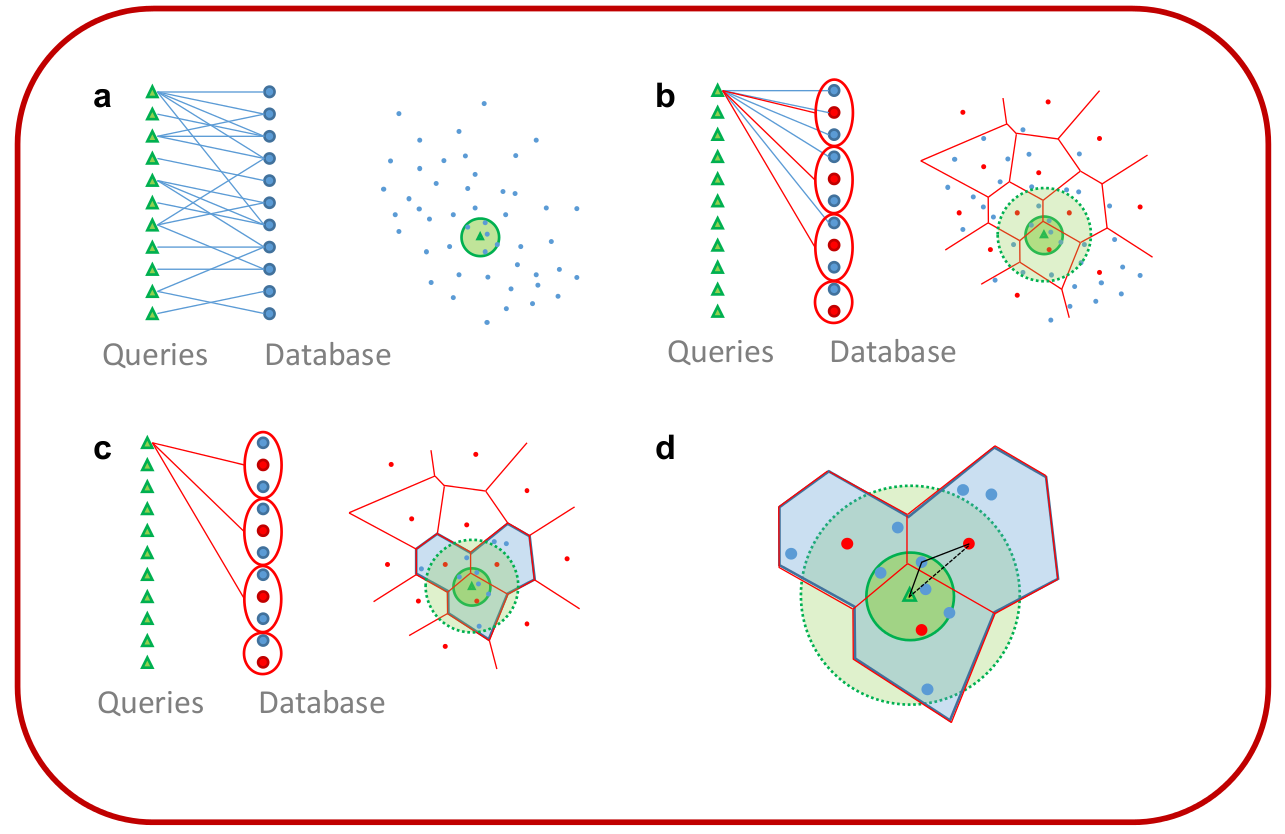
\includegraphics[width=8in]{assets/dataStructure.png}}
    \caption{ Entropy-scaling data structure for similarity search. %
            (a) The na\"ive approach tests each query against each database entry to find entries within distance $r$ of the query (inside the small green disc). %
            (b) By selecting appropriate cluster centers with maximum radius $r_c$ to partition the database, we can (c) first do a coarse search to find all cluster centers within distance $r+r_c$ of a query (larger green disc), %
 and then the (d) triangle inequality guarantees that a fine search over all corresponding cluster entries (blue polygonal regions) will suffice.}
    \label{fig:dataStructure}
\end{figure}

%We present here an opportunistic data structure for similarity search that scales with the entropy of the underlying database.
In the following we consider entropy to be nearly synonymous with distance between points in a high-dimensional space.
For genomic sequences, this can be edit distance; for chemical graphs, Tanimoto 
distance; and for general vectors, Euclidean or cosine distance.
We are interested in the similarity search problem of
finding all points in a set that are close to (i.e., similar to) the query point.
The basics of the data structure itself are presented in Figure \ref{fig:dataStructure}, but here we provide conceptual motivation.

Let us first consider what it means for a large biological data set, considered as points in a high-dimensional space, to be highly redundant.
Perhaps many of the points are exact duplicates; this easy scenario is trivially exploited by de-duplication and is already standard practice, such as
the NR NCBI protein database \cite{pruitt2005ncbi}.
Or maybe the points mostly live on a low-dimensional subspace; statistical tools such as Principal Component Analysis exploit this property in data analysis.
Furthermore, if the dimension of the subspace is sufficiently low,
it can be divided into cells, allowing quick similarity searches by looking only at nearby cells \cite{weber1998quantitative}.
However, when the dimensionality of the subspace increases, cell search time 
grows exponentially; additionally, in sparse data sets, most of the cells will 
be empty, which wastes search time.

\begin{figure}[p]
    \vspace{-5em}
    \centering
    \centerline{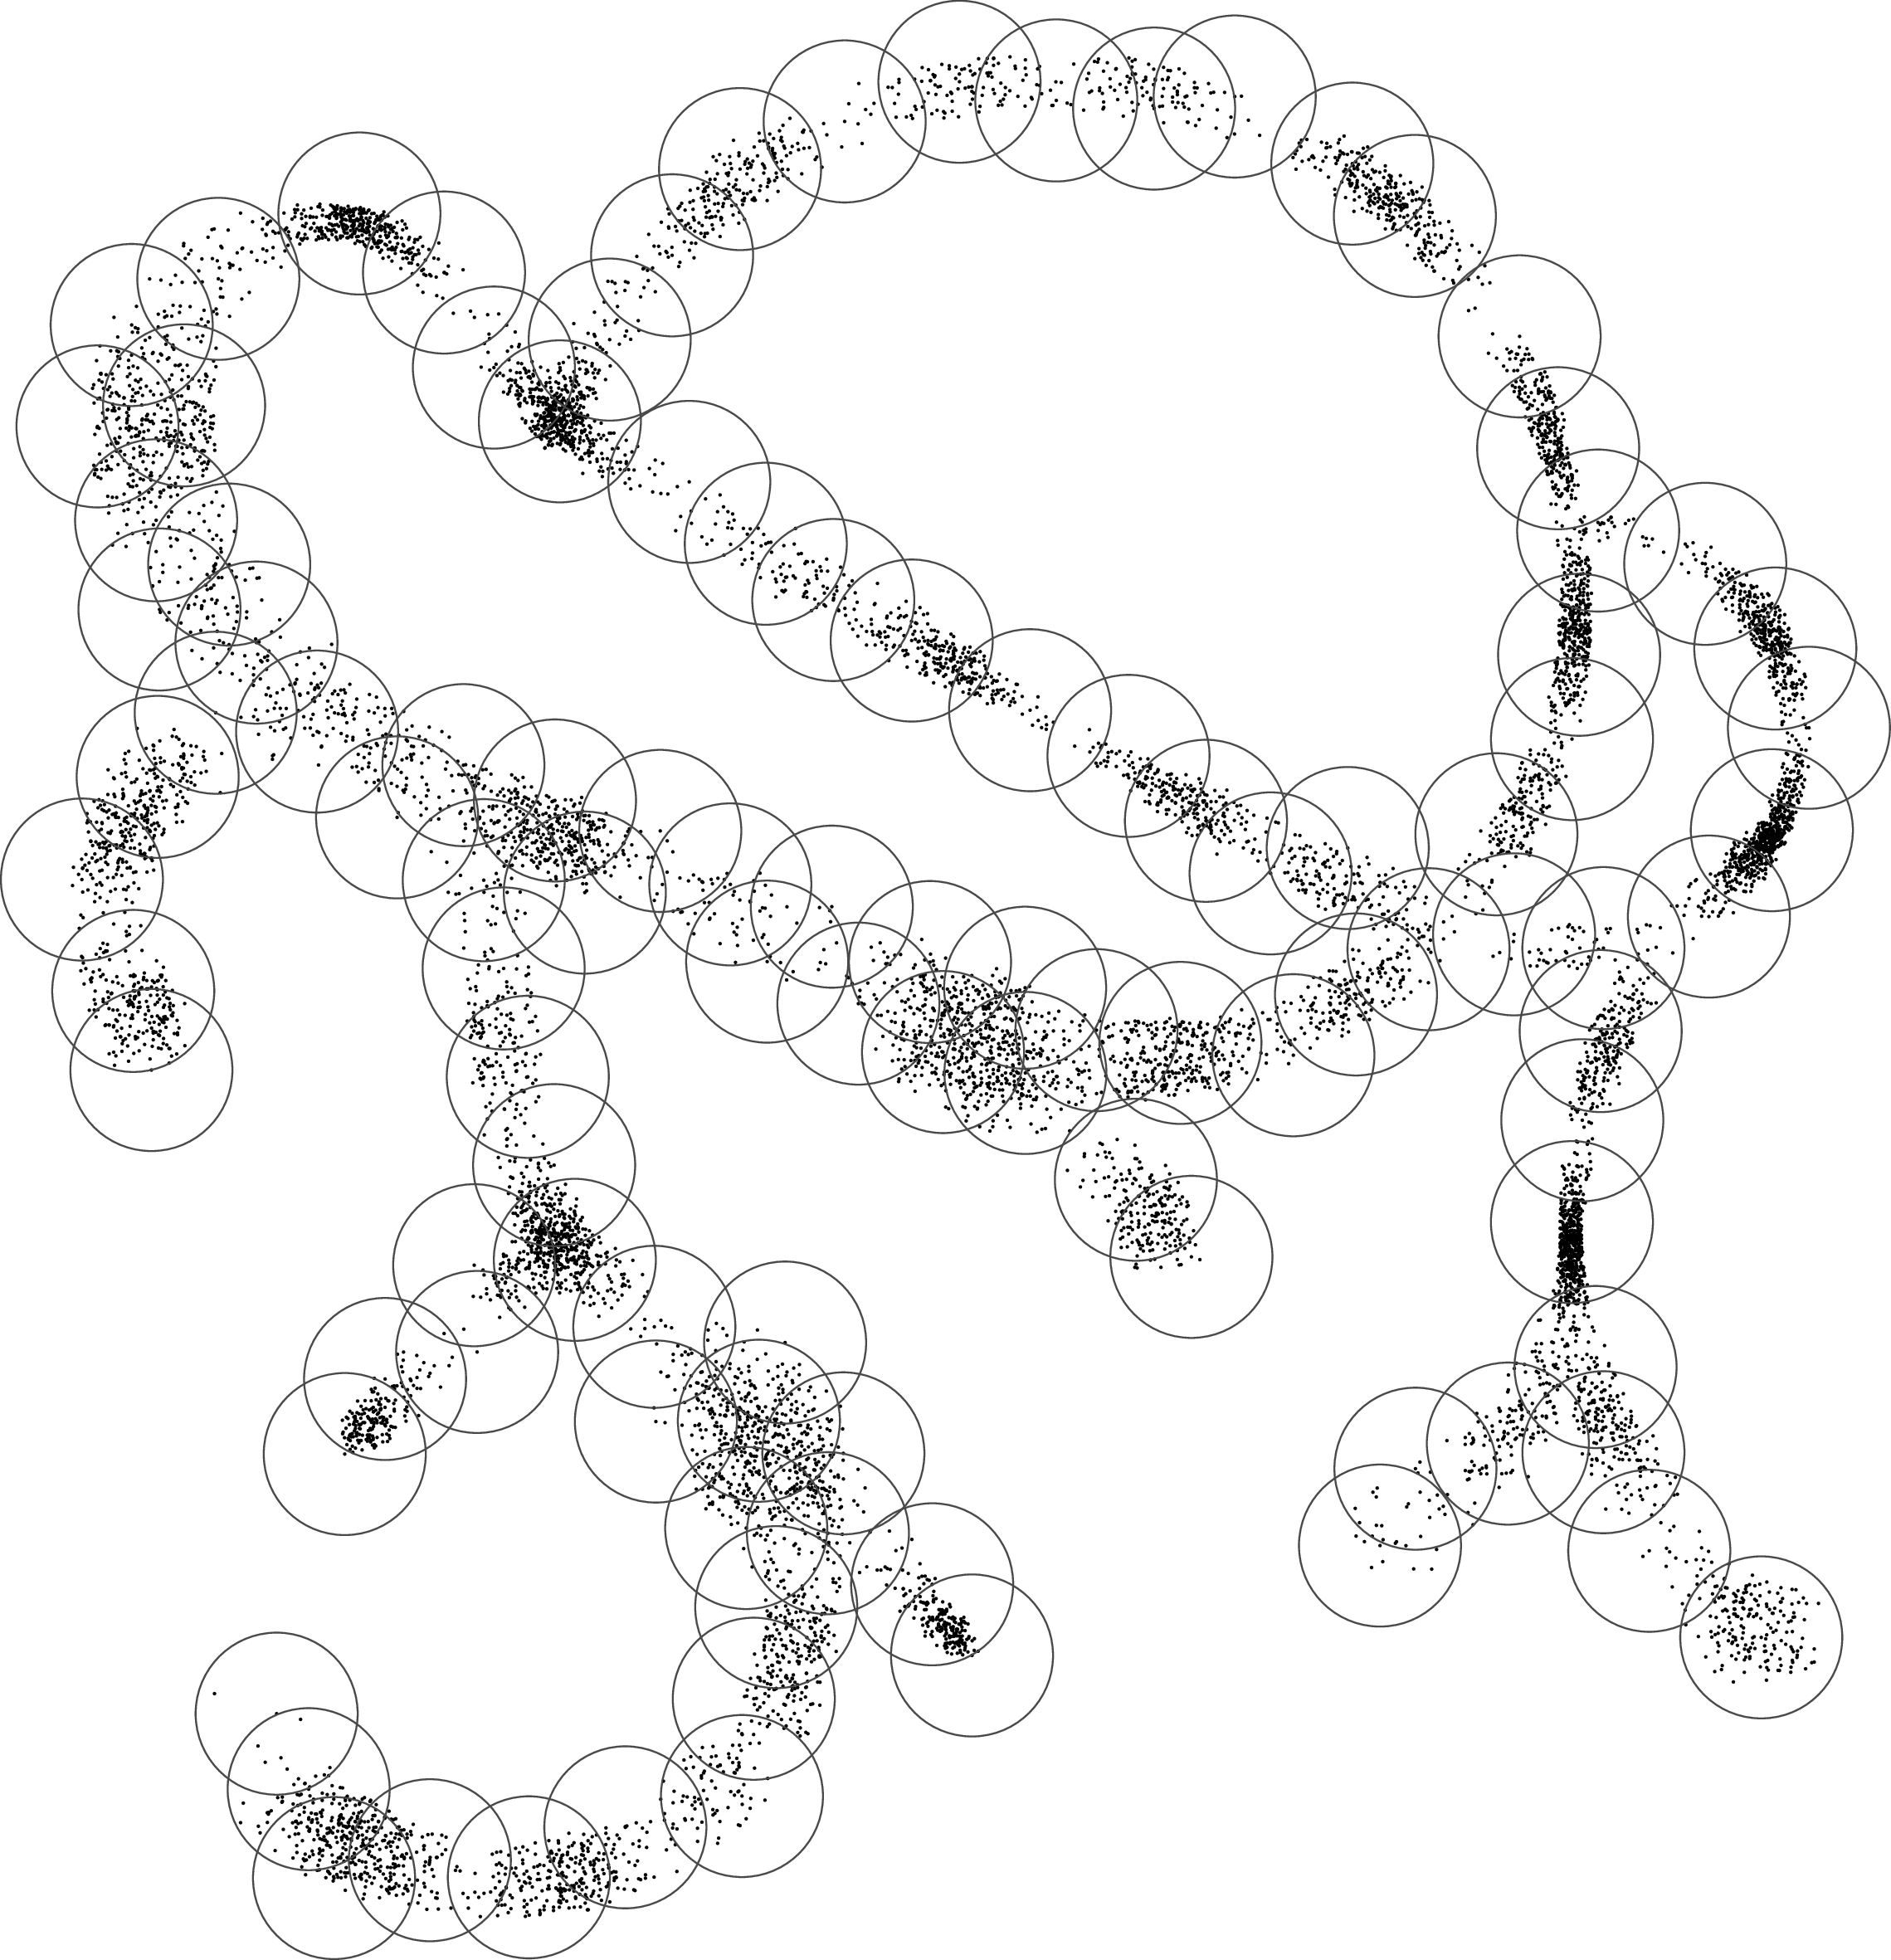
\includegraphics[width=8in]{assets/treepoints/treepoints2D_clusters.png}}
    \caption{Cartoon depiction of points in an arbitrary high-dimensional space that live close to a 1D tree-like structure, as might arise from genomes generated by mutation and selection along an evolutionary tree of life. 
Although high-dimensional at a fine scale, at the coarser scale of covering spheres, the data cloud looks nearly 1-dimensional, which enables entropy-scaling of similarity search. The cluster center generation was performed using the same method we used for protein structure search.}
    \label{fig:tree}
\end{figure}

More importantly, biological data sets generally do not live in low-dimensional subspaces.
Consider the instructive case of genomes along an evolutionary `tree of life' (Figure \ref{fig:tree}).
Such a tree has many branches (though admixture merges branches back together),
and looks nearly 1-dimensional locally, but it is globally of higher dimension.
Additionally, because of diffusion due to mutation, each of the branches is also `thick' (high-dimensional) when looked at closely.
Viewing this example as a low-dimensional \textit{subspace}, as in PCA, is 
incorrect.

However, the local low-dimensionality can be exploited by looking on the right scales: a coarse scale in which the tree looks 1-dimensional locally and a fine scale where the branch width matters.
We cover the tree with spheres of radius $r_c$, where $r_c$ is on the order of the branch width; these spheres determine our clusters, and the number of them is the metric entropy of the tree \cite{tao2008product}.
Because all the points within a sphere are close to each other, they are highly 
redundant and can be encoded in terms of one another, saving space.

By the triangle inequality, in order to search for all points within distance $r$ of a query we need only look in nearby spheres with centers (i.e., representatives) within a distance $r+r_c$ of the query (Figure \ref{fig:dataStructure}d).
%ref Figure 1?.
However, because the spheres have radius comparable to branch width, the tree is locally 1-dimensional on the coarse scale; we will call this the fractal dimension $d=1$ of the tree at the scale $r_c$ \cite{falconer1990fractal}, where $r_c$ is essentially our ruler size.
Thus, increasing the search radius for coarse search only linearly increases the number of points that need to be searched in a fine search.

A similar analysis holds in the more general case.
Given a database with fractal dimension $d$ and metric entropy $k$ at the scale $r_c$, we show in the Supplemental Methods that the time-complexity of similarity search on database $D$ for query $q$ with radius $r$ is
\begin{gather*}
    O\Bigg(
    \underbrace{k}_{\textrm{metric entropy}} +
    \overbrace{\left|B_D(q,r)\right|}^{\textrm{output size}}
    \underbrace{\left(\frac{r+2r_c}{r}\right)^d}_{\textrm{scaling factor}}
     \Bigg) .
\end{gather*}
Thus, for small fractal dimension and output size, similarity search is asymptotically linear in metric entropy.
Additionally, because the search has to look at only a small subset of the clusters, the clusters can be stored in compressed form, and only decompressed as needed, giving space savings that also scale with entropy.
As an aside, note that the space-complexity actually scales with the sum of metric and information-theoretic entropy, rather than just metric entropy 
(Supplemental Methods: Theory).
%Similarly, using these covering spheres, the database can be stored in a 
%compressed manner (see Supplemental Methods for further details).

Entropy-scaling data structures can be expected to provide a boost to 
approximate search when fractal dimension is low (i.e., close to 1) and metric
entropy is low.
Specifically, the ratio $\frac{|D|}{k}$ provides an estimate of the acceleration factor
for just the coarse search component compared to a full linear search.
Local fractal dimension around a data point can be computed by determining the
number of other data points within two radii $r_1$ and $r_2$ of that point;
given those point counts ($n_1$ and $n_2$, respectively), fractal dimension $d$
is simply $d=\frac{\log (n_2 / n_1)}{ \log (r_2 / r_1)}$.
Sampling this property over a dataset can provide a global average fractal 
dimension; low fractal dimension will indicate that fine search time will not
obviate the gains provided by an entropy-scaling data structure.

We have presented the simplest such data to analyze for clarity of exposition.
However, real data is generally messier.
Sometimes the distance function is not a metric, so we lose the triangle inequality guarantee of 100\% sensitivity;
sometimes different distance functions can be used for the clustering versus search;
and sometimes even what counts as a distinct data point is not entirely clear without domain knowledge (for example, long genomic sequences might be better broken into shorter subsequences).

We show in the following that entropy-scaling data structures are robust to the variations presented by real data.
Through the diversity of the applications we explore in this paper, we demonstrate that the general scheme works for massively accelerating similarity search in a set of different contexts.
These applications are enabled by augmenting the data structure with domain-specific distance functions in different stages of the algorithm, as well as preprocessing to take advantage of domain-specific knowledge.
We expect that so long as the data set exhibits both low entropy and low 
fractal dimension---and this is empirically true in biological systems---our 
entropy-scaling data structure has the potential to achieve massive speedup 
over more na\"ive methods and significant speedup over even other highly 
optimized methods.

\subsection{Application to high-throughput drug screening}

Chemogenomics is the study of drug and target discovery by using chemical
compounds to probe and characterize proteomic 
functions~\cite{bredel2004chemogenomics}.
Particularly in the fields of drug discovery and drug repurposing, prediction 
of biologically active compounds is a critical task. 
Computational high-throughput screening can eliminate many compounds from 
wet-lab consideration, but even this screening can be time-consuming.
PubChem~\cite{bolton2008pubchem}, a widely-used repository of molecular compound 
structures, 
has grown greatly since 2008. 
In July 2007, PubChem contained 10.3 million compounds.
In October 2013, PubChem contained roughly 47 million compounds, while
in December 2014 it contained 61.3 million compounds.

We designed this compression and search framework around one of the standard 
techniques for high-throughput screening of potential drug compounds, the use 
of maximum common subgraph (MCS) to identify similar motifs among molecules \cite{cao2008maximum, rahman2009small}.
We introduce Ammolite, a method for clustering molecular databases such as 
PubChem, and for quickly searching for 
similar molecular structures in compressed space.
Ammolite demonstrates that entropy-scaling methods can be extended to data types that are not inherently sequence based.
Ammolite is a practical 
tool that provides approximately a factor of 10 speed-up with greater than 95\% accuracy compared to the popular SMSD~\cite{rahman2009small}.

MCS-based search of molecule databases typically matches pairs of molecules by 
Tanimoto distance~\cite{rahman2009small}. 
Tanimoto distance obeys the triangle inequality, and is more useful in the 
domain of molecular graphs than other
distance metrics such as graph distance \cite{bunke1998graph}.

To compress a molecule database, we project the space of small molecules onto a subspace by removing nodes and edges that do not participate in simple cycles
(Figure S1).
Clusters are exactly pre-images of of this projection operator (i.e.,~all molecules that are isomorphic after simplification form a cluster).
Coarse search is performed by finding the MCS on this much smaller projection subspace. This increases speed by reducing both the required number of MCS operations 
and the time required for each MCS operation, which scales with the size of the molecule.
It is worth noting that this pre-processing of molecular graphs can cause the 
triangle inequality to be violated; while the distance function is a metric, the
clustering does not respect that metric.
Ammolite can be readily plugged in to existing analysis pipelines for 
high-throughput drug screening.

Our entropy-scaling data structure can be applied to PubChem because it has both low fractal
dimension and low metric entropy.
In particular, we determined the mean local fractal dimension of PubChem to be 
approximately 0.2 in the neighborhood between 0.2 and 0.4 Tanimoto distance,
and approximately 1.9 in the neighborhood between 0.4 and 0.5.
The expected speedup is measured by the ratio of database size to metric entropy, which for PubChem is approximately 11:1.

Because SMSD is not computationally tractable on the entire PubChem database,
we benchmarked Ammolite against SMSD on a subset of 1 million molecules from PubChem.
Since SMSD's running time should scale linearly with the size of the database, we extrapolated the
running time of SMSD on a subset of 10 million molecules, as well as on the entire PubChem database.
For these benchmarks, we used three query molecules with at least two cyclohexane rings, namely PubChem IDs 28250541, 1504670, and 23743178.
We also used SMSD as a gold standard against which we measured Ammolite's recall.
As shown in Table~\ref{ammo1m}, Ammolite achieves at least 96\% recall with respect to SMSD.
Furthermore, as shown in Tables~\ref{ammo10m} and \ref{ammo47m}, Ammolite's speed gains with respect to SMSD grow as the database grows.
Figure~\ref{fig:ammoscale} illustrates this scaling for one query.

\begin{table}
\caption{Benchmarks of Ammolite vs. SMSD on databases of (a) 1 million molecules (b) 10 million molecules (c) All of PubChem (47 million molecules)}


\begin{subtable}{1\textwidth}
\caption{Ammolite benchmark on database of 1 million molecules}
\label{ammo1m}
\begin{tabular}{ccccc}
\hline
PubChem ID & SMSD (hours) & Ammolite (hours) & Speedup & Recall \\
\hline
28250541 & 43.3 & 12.2 & 3.5 & 100\% \\
\hline
1504670 & 8.1 & 3.6 & 2.3 & 96.3\% \\
\hline
23743178 & 21.7 & 2.7 & 8.2 & 100\% \\
\hline
\end{tabular}
\end{subtable}

\vspace{1em}

\begin{subtable}{1\textwidth}
\caption{Ammolite benchmark on database of 10 million molecules}
\label{ammo10m}
\begin{tabular}{ccc}
\hline
PubChem ID & Ammolite (hours) & Speedup \\
\hline
28250541 & 97.7 & 3.2 \\
\hline
1504670 & 25.4 & 4.4 \\
\hline
% 23743178 & 1. & 10.2 \\
% \hline
\end{tabular}
\end{subtable}

\vspace{1em}

\begin{subtable}{1\textwidth}
\caption{Ammolite benchmark on entire PubChem database}
\label{ammo47m}
\begin{tabular}{ccc}
\hline
PubChem ID & Ammolite (hours) & Speedup \\
% \hline
% 28250541 & 14423 & 21 \\
% \hline
% 1504670 & 3235 & 123 \\
\hline
23743178 & 81.5 & 12.5 \\
\hline
\end{tabular}
\end{subtable}
\end{table}

\begin{figure}[hbp]
    \centering
    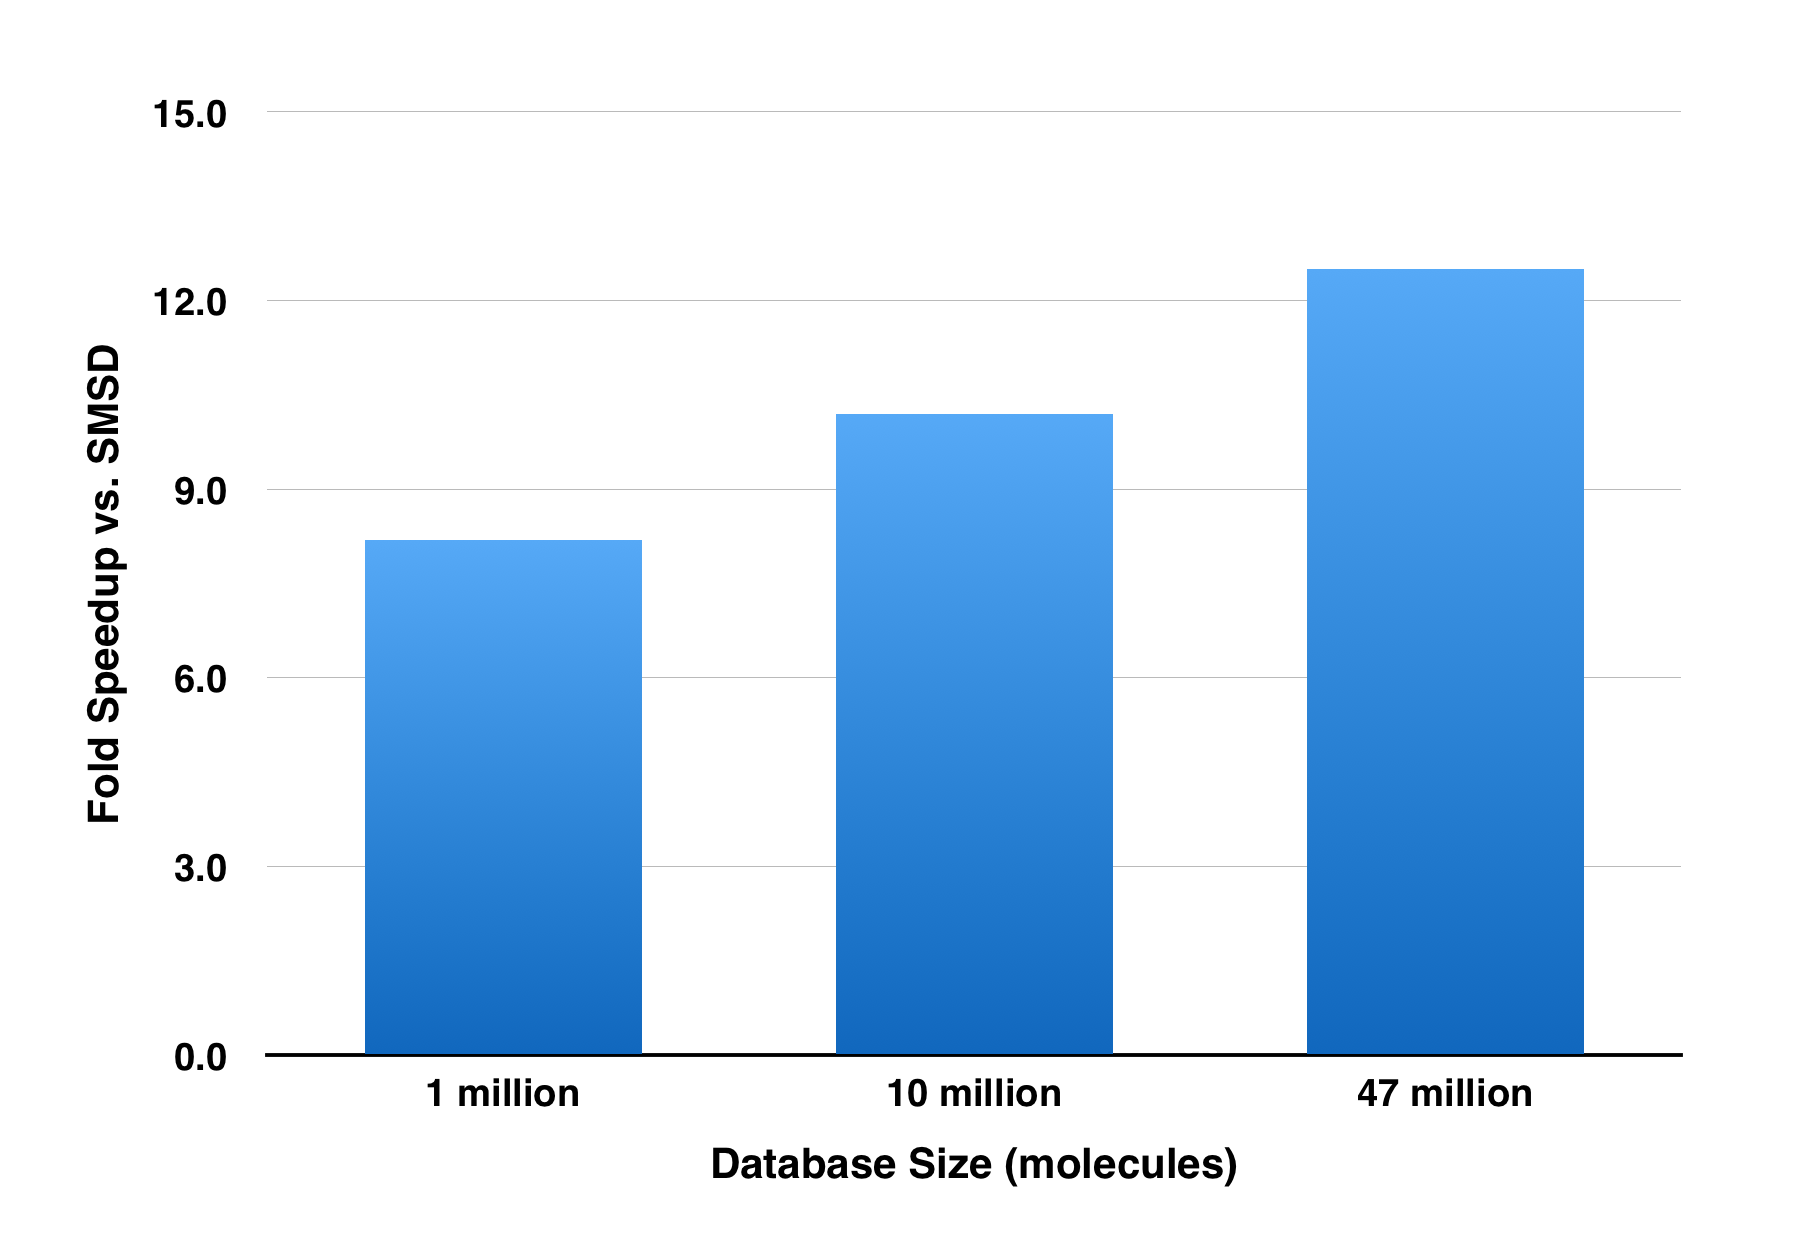
\includegraphics[width=1\textwidth]{assets/ammolite-speedup.png}
    \caption{ Ammolite's speedup over SMSD. On PubChem ID 23743178,
    Ammolite's gains overs SMSD increase with database size, achieving a 12.5x
    speedup on the full PubChem from October, 2013, which contains 47 million 
    compounds.
    }
    \label{fig:ammoscale}
\end{figure}

\subsection{Application to metagenomics}

Metagenomics is the study of genomic data sequenced directly from environmental
samples.
It has led to improved understanding of how ecosystems recover
from environmental damage~\cite{tyson2004community} and how the human gut responds 
to diet
and infection~\cite{david2014host}.
Metagenomics has even provided some surprising insights into disorders 
such as Autism Spectrum Disorder~\cite{macfabe2012short}.

BLASTX~\cite{altschul1990basic} is widely used in metagenomics to map
reads to protein databases such as KEGG~\cite{kanehisa2000kegg} and NCBI's 
NR~\cite{sayers2011database}.
This mapping is additionally used as a primitive in pipelines such as MetaPhlAn~\cite{segata2012metagenomic}, 
PICRUSt~\cite{langille2013predictive}, and MEGAN~\cite{huson2011integrative} to
determine the microbial composition of a sequenced sample.
Unfortunately, BLASTX's run time requirements scale linearly with the product 
of the size of the full read dataset and the targeted protein database, and 
thus each year require exponentially more runtime to process the exponentially 
growing read data. 
These computational challenges are at present a barrier to widespread use of 
metagenomic data throughout biotechnology, which constrains genomic medicine 
and environmental genomics~\cite{frank2008gastrointestinal}.
For example, \citet{mackelprang2011metagenomic} reported that using BLASTX to map 246
million reads against KEGG required 800,000 CPU hours at a supercomputing 
center.

Although this is a problem already for major research centers, it is especially
limiting for on-site analyses in more remote locations.
In surveying the 2014 Ebola outbreak, scientists physically shipped samples on 
dry ice to Harvard for sequencing and analysis \cite{gire2014genomic}.
Even as sequencers become more mobile, lack of fast Internet connections in remote
areas can make it impossible to centralize and expediate processing (viz.: the cloud);
local processing on resource-constrained machines remains essential.
Thus, a better-scaling and accurate version of BLASTX raises the possibility of 
not only faster computing for large research centers, but also of performing
entirely on-site sequencing and metagenomic analyses.

We have applied our entropy-scaling data structure to the problem of 
metagenomic search and demonstrate caBLASTX, a method whose software 
implementation provides an acceleration of BLASTX by a factor of up 
to 673.
This application illustrates the potential of entropy-scaling data structures, while
providing a useful tool for metagenomic research.
It can be readily plugged in to existing analysis pipelines (e.g. for microbial 
composition analysis using MEGAN).

CaBLASTX is useful for two of the most common metagenomic analysis tasks. 
The first of these is mapping short nucleotide reads generated by next-generation sequencing technology to a protein database,
while the second is mapping assembled or partially-assembled
nucleotide sequences.
In the former instance, there is typically high coverage of the metagenomes
being sequenced, ranging from 30x to 200x coverage.
CaBLASTX takes advantage of this redundancy
by clustering the read set as well, obtaining an additional speed gain that is
proportional to the amount of redundancy in the read data.
We note that this query-side clustering is in addition to the entropy-scaling
framework as described and the run-time cost of clustering queries cannot
be amortized over future queries, so
we expect this enhancement to provide a 
constant factor improvement.

Our entropy-scaling data structure can be applied to the NCBI's NR database because it, 
like PubChem, exhibits low fractal dimension and metric entropy.
We determined the mean local fractal dimension of the NCBI's NR database, using 
sequence identity of alignment as a distance function, to be approximately 1.6 
in the neighborhood between 70\% and 80\% protein sequence identity.
The ratio of database size to metric entropy, which gives an indicator of expected speedup,
is approximately 30:1.
Indeed, the notion that protein sequence space exhibits structure, 
and lends itself to clustering, has precedent~\cite{linial1997global}.

To evaluate the run-time performance of caBLASTX, we tested it against
BLASTX and two other top performing tools: RapSearch2~\cite{zhao2012rapsearch2} and the recently-released
Diamond~\cite{buchfink2014fast}.
On a large-scale publicly-available database (Supplemental Methods), we found that caBLASTX provides substantial runtime improvements 
(although similar to Diamond) at greater accuracy (Table~\ref{mgspeed}).
Notably, the running time for BLASTX was 14,423 minutes, 
while caBLASTX took 21 minutes, a speedup of 673x.

CaBLASTX also sped up BLASTX in aligning assemblies thought to be exons to a protein
database, in which case metagenomic reads have already been 
assembled (Table~\ref{mgspeed}).
We benchmarked caBLASTX vs. BLASTX on a dataset consisting of 22,778 assemblies
from human gut microbiota, 3.1 megabases in total, searching against the NCBI's
`NR' non-redundant protein database from September, 2014.
The running time of BLASTX was 3235 minutes, compared to 123 minutes for 
caBLASTX, a speedup of 26.3.
In this instance, the query-side clustering of caBLASTX is not applicable, so
the performance gains are more modest.
For both next-generation sequencing (NGS) reads and assemblies, Diamond had slightly faster running time than caBLASTX, albeit at the expense of accuracy, while RapSearch2 was slower.

\begin{table}
\caption{(a) Running time and (b) accuracy of BLASTX, caBLASTX, RapSearch2, and Diamond}
\begin{subtable}{1\textwidth}
\caption{Running time}
\label{mgspeed}
\begin{tabular}{ccccc}
\hline
dataset & BLASTX & caBLASTX & RapSearch2 & Diamond \\
\hline
NGS reads (sec) & 14423 & 21 & 51 & 13 \\
\hline
assemblies (sec) & 3235 & 123 & 194 & 50 \\
\hline
\end{tabular}
\end{subtable}

\begin{subtable}{1\textwidth}
\caption{Accuracy against BLASTX}
\label{mgacc}
\begin{tabular}{ccccc}
\hline
dataset & BLASTX & caBLASTX & RapSearch2 & Diamond \\
\hline
NGS reads & 100\% & 95.7\% & 79.5\% & 76.9\% \\
\hline
assemblies & 100\% & 99.2\% & 87.7\% & 91.0\% \\
\hline
\end{tabular}
\end{subtable}
\end{table}

As shown in Table~\ref{mgacc}, caBLASTX achieves substantially better accuracy
than other methods: 99.2\% accuracy on assemblies and 95.7\% 
accuracy even on the raw reads.
Experiments validating accuracy treated BLASTX as a gold standard. 
Since caBLASTX accelerates BLASTX
using entropy-scaling techniques, false positives with respect to BLASTX are 
not possible, but false negatives are.
We compared the hits from BLASTX and caBLASTX on the same human gut
assemblies and raw reads used for benchmarking, in order to evaluate the accuracy when
query-side compression is not used.
As false positive hits with respect to BLASTX are not possible, we report as 
accuracy the fraction of BLASTX hits that are also returned by caBLASTX.

While Diamond is somewhat faster than caBLASTX, its running time still scales
linearly with database size.
In contrast, as an entropy-scaling search, caBLASTX will demonstrate greater
acceleration as database sizes grow~\cite{daniels2013compressive}.
Furthermore, Diamond achieves its constant acceleration at the expense of 
accuracy, particularly on raw reads.
Moreover, caBLASTX accelerates standard BLASTX itself, and allows the
user to pass arbitrary parameters to the underlying BLASTX during fine search.
Thus, caBLASTX may be suitable for a wider variety of existing analysis 
pipelines.

\subsection{Application to protein structure search}

The relationship between protein structure and function has been a subject of intense study for decades,
and this strong link has been used for the prediction of function from structure \cite{hegyi1999relationship}.
Specifically, given a protein of solved (or predicted) structure but unknown function, the efficient identification
of structurally similar proteins in the Protein Data Bank (PDB) is critical to function prediction.
Relatedly, finding structural neighbors can also give insight into the evolutionary origins of proteins of interest \cite{yona1999protomap,nepomnyachiy2014global}.

One approach to finding structural neighbors is to attempt to align the query protein to all the entries in the PDB using a structural aligner, such as 
STRUCTAL \cite{subbiah1993structural}, ICE \cite{shindyalov1998protein}, or 
Matt \cite{menke2008matt}.
However, performing a full alignment against every entry in the PDB is prohibitively expensive, especially as the database grows.
To mitigate this, \citep{budowski2010fragbag} introduced the tool FragBag, which avoids performing full alignments but rather describes each protein as a
`bag of fragments,' where each fragment is a small structural motif.
FragBag has been reported as comparable to structural aligners such as STRUCTAL or ICE,
and its bag-of-fragments approach
allows it to perform comparisons much faster than standard aligners.
Importantly for us, the bag of fragments is just a frequency vector, making
FragBag amenable to acceleration through entropy-scaling.

By first verifying that the local fractal dimension of PDB FragBag frequency vectors is low in most regimes ($d \approx 2-3)$, Figure S3), we are given reason to think that this problem is amenable to entropy-scaling search.
As an estimate of potential speedup, the ratio of PDB database size to metric 
entropy at for the chosen cluster radii is on average approximately 10:1.
We directly applied our entropy-scaling data structure without any additional 
augmentation: esFragBag (entropy-scaling FragBag) is able to achieve an average
factor of 10 speedup of the highly-optimized FragBag with less than 0.2\% loss 
in sensitivity and no loss in specificity.

For this last example, we intentionally approach the application of entropy-scaling data structures to FragBag in a blind manner,
without using any domain-specific knowledge.
Instead, we use the very same representation (bag of fragments) and distance functions (Euclidean and cosine distances)
as FragBag, coupled with a greedy k-centers algorithm to generate the clustered representation.
Note that this is in stark contrast to caBLASTX and Ammolite, which both exploit domain knowledge to further improve performance.
Thus, esFragBag only involves extending an existing codebase with new database generation and similarity search functions.

We investigate the increases in speed resulting from directly applying the entropy-scaling data structure for both Euclidean and cosine distances and found the acceleration is highly dependent on both the search radius and cluster radius (Figure \ref{fig:fragbag}).
For cosine distance, we generated databases with maximum cluster radii of 0.1, 0.2, 0.3, 0.4, and 0.5.
Then, for each query protein from the set \{\texttt{4rhv}, \texttt{1ake}, \texttt{1bmf}, \texttt{1rbp}\} (identified by PDB IDs), we ran both na\"ive and accelerated similarity searches with radii of $0.02i, \forall i \in \{0,\ldots,49\}$.
This test was repeated 5 times for each measurement, and the ratio of average accelerated vs na\"ive times is shown in Figure \ref{fig:fragbag_cosine}.
For Euclidean distance, we generated databases with maximum cluster radii of 10, 20, 25, 50, and 100.
Again, for each query protein drawn from the same set, we compared the average over 5 runs of the ratio of average accelerated vs na\"ive times (Figure \ref{fig:fragbag_euclid}).

Not only is the acceleration highly dependent on both the search radius $r$ and the maximum cluster radius $r_c$,
but the choice of query protein also affects the results.
We suspect that this effect is due to the geometry of protein fragment frequency space being very `spiky' and `star-like'.
Proteins that are near the core (and thus similar to many other proteins) show very little acceleration when our data structure is used because the majority of the database is nearby, whereas proteins in the periphery have fewer neighbors and are thus found much more quickly.
Changing the maximum cluster radius effectively makes more proteins peripheral proteins, but at the cost of overall acceleration.

Naturally, as the search radius expands, it quickly becomes necessary to compare against nearly the entire database, destroying any acceleration.
For the cosine space in particular, note that the maximum distance between any two points is $1$, so once the coarse search radius of $r+r_c \ge 1.0$, there cannot ever be any acceleration as the fine search encompasses the entire database.
Similarly, once the coarse search encompasses all (or nearly all) the clusters in Euclidean space, the acceleration diminishes to 1x, and the overhead costs make the entropy-scaling data structure perform worse than a na\"ive search.
However, as we are most interested in proteins that are very similar to the query, the low-radius behavior is of primary interest.
In the low-radius regime, esFragBag demonstrates varying though substantial acceleration (2-30x, averaging $>$10x for both distance functions for the proteins chosen) over FragBag.

It is instructive to note that because of the very different geometries of Euclidean vs cosine space, acceleration varies tremendously for some proteins, such as \texttt{4rhv} and \texttt{1bmf}, which display nearly opposite behaviors.
Whereas there is nearly 30x acceleration for \texttt{4rhv} in cosine space for low radius, and the same for \texttt{1bmf} in Euclidean space, neither achieves better than $\sim$ 2.5x acceleration in the other space.

\begin{figure}[p]
    \centering
    \vspace{-10em}
    \centerline{
    \begin{subfigure}[b]{3.4in}
        \caption{Cosine distance}
        \label{fig:fragbag_cosine}
        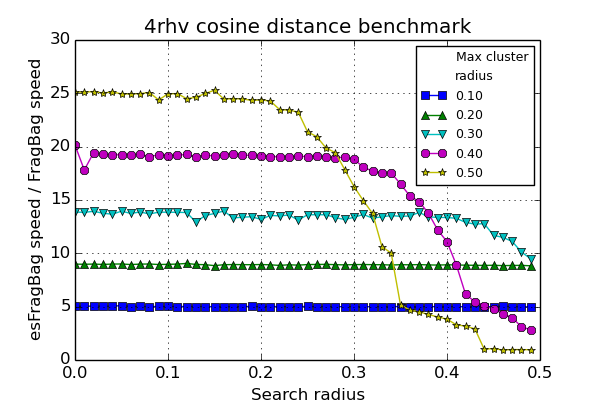
\includegraphics[width=1\textwidth]{assets/4rhv_cosine.png}
    \end{subfigure}%
    \begin{subfigure}[b]{3.4in}
        \caption{Euclidean distance}
        \label{fig:fragbag_euclid}
        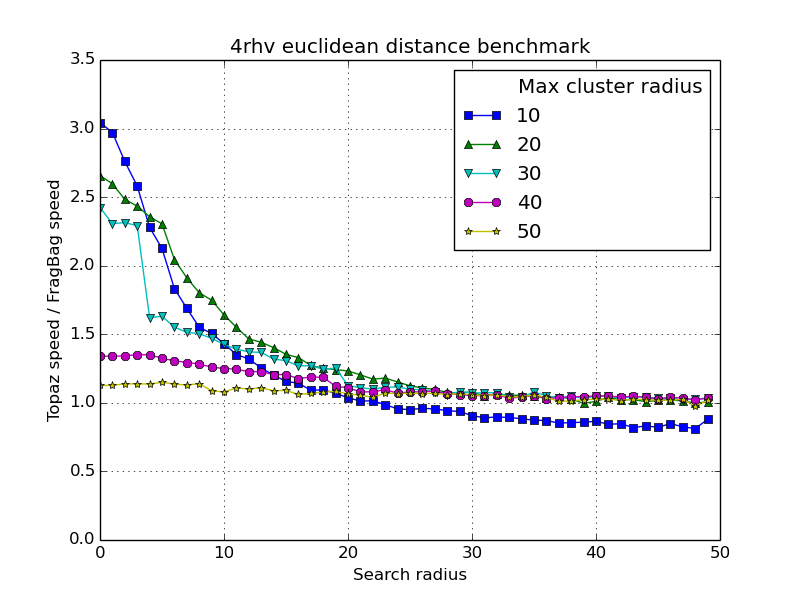
\includegraphics[width=1\textwidth]{assets/4rhv_euclid.png}
    \end{subfigure}
    }
    \centerline{
    \begin{subfigure}[b]{3.4in}
        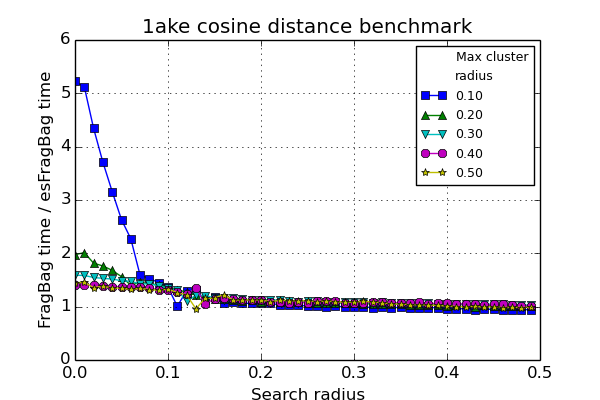
\includegraphics[width=1\textwidth]{assets/1ake_cosine.png}
        %\caption{}
    \end{subfigure}%
    \begin{subfigure}[b]{3.4in}
        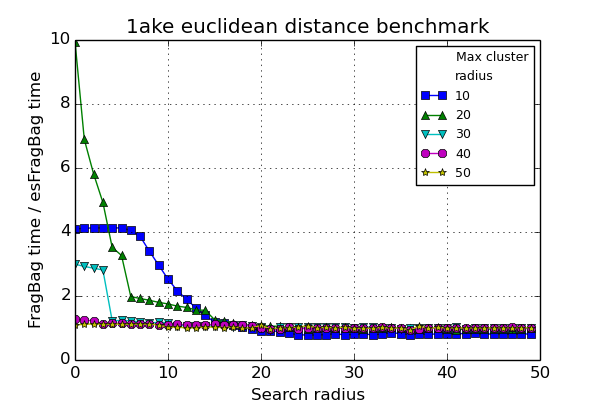
\includegraphics[width=1\textwidth]{assets/1ake_euclid.png}
        %\caption{}
    \end{subfigure}
    }
    \centerline{
    \begin{subfigure}[b]{3.4in}
        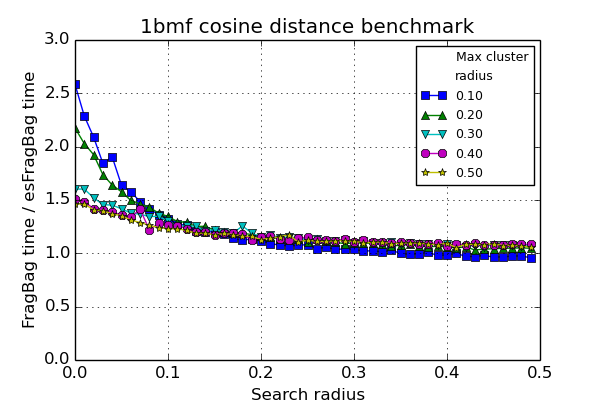
\includegraphics[width=1\textwidth]{assets/1bmf_cosine.png}
        %\caption{}
    \end{subfigure}%
    \begin{subfigure}[b]{3.4in}
        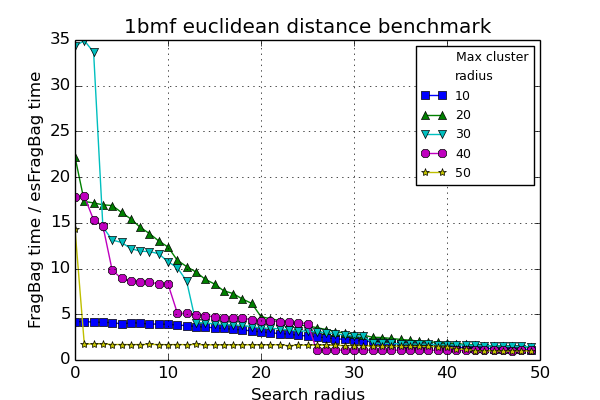
\includegraphics[width=1\textwidth]{assets/1bmf_euclid.png}
        %\caption{}
    \end{subfigure}
    }
    \centerline{
    \begin{subfigure}[b]{3.4in}
        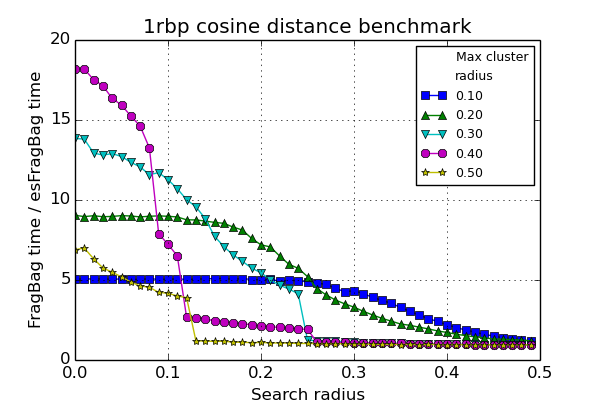
\includegraphics[width=1\textwidth]{assets/1rbp_cosine.png}
        %\caption{}
    \end{subfigure}%
    \begin{subfigure}[b]{3.4in}
        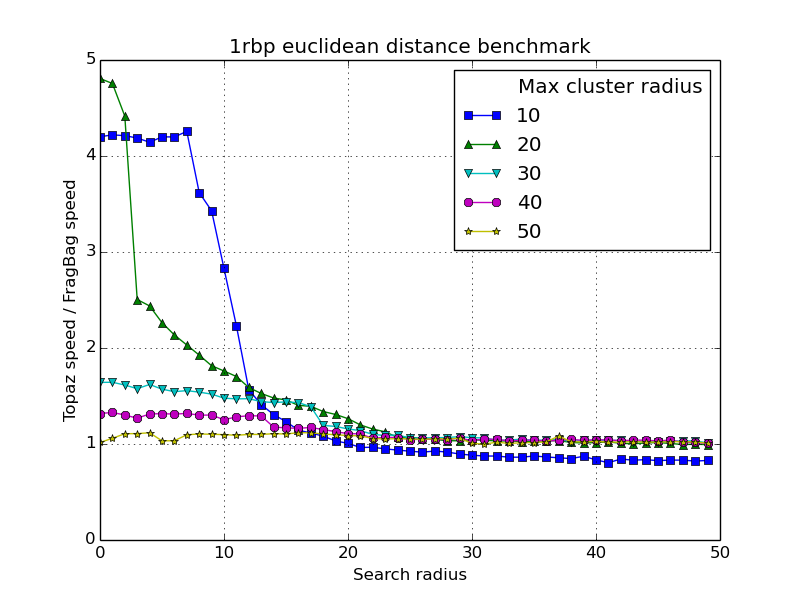
\includegraphics[width=1\textwidth]{assets/1rbp_euclid.png}
        %\caption{}
    \end{subfigure}
    }
    \caption{Scaling behavior of esFragBag. EsFragBag benchmarking data with parameters varied until the acceleration advantage of esFragBag disappears. As search radius increases, the fraction of the database returned by the coarse search increases, ultimately returning the whole database. Unsurprisingly, when returning the whole database in the coarse search results, there are no benefits to using entropy-scaling data structures. (a) Cosine distance gives on the whole better acceleration, but results in $>99.8\%$ sensitivity, whereas (b) Euclidean distance as a metric is guaranteed by the Triangle Inequality to get $100\%$ sensitivity.}
    \label{fig:fragbag}
\end{figure}

Finally, while Euclidean distance is a metric---for which the triangle inequality guarantees 100\% sensitivity---cosine distance is not.
Empirically, however, for all of the queries we performed, we achieve $> 99.8\%$ sensitivity (Table \ref{tab:fragbag_cosine_sensitivity}).
%Full results for each data point can be found in supplementary data files.

\begin{table}
    \centering
    \caption{Average sensitivity of esFragBag compared to FragBag when using cosine distance for the trials described in Figure \ref{fig:fragbag_cosine}. This table averages the sensitivities for each choice of search radii $\{0, 0.01, \ldots, 0.49\}$. (NB: no analogous table is given for Euclidean distance as the Triangle Inequality ensures perfect recall).}
    \label{tab:fragbag_cosine_sensitivity}
    \begin{tabular}{|c|cccc|}
        \hline
        \backslashbox{Cluster radii}{Query protein}  & 4rhv & 1ake & 1bmf & 1rbp \\
        \hline
        0.10  & 1  & 0.999840     & 0.998490 & 0.999950  \\
        0.20  & 1  & 0.999918     & 0.999001 & 0.999978  \\
        0.30  & 1  & 0.999926     & 0.999649 & 1  \\
        0.40  & 1  & 0.999974     & 0.999796 & 1  \\
        0.50  & 1  & 0.999984     & 0.999934 & 1  \\
        \hline
    \end{tabular}
\end{table}

\section{Discussion}

\textbf{The primary advance of entropy-scaling data structures is that they bound both time and space as functions of the data set entropy (albeit using two different notions of entropy).}
In this paper, we have introduced an entropy-scaling data structure for accelerating approximate search,
allowing search on large omics data sets to scale even as those data sets grow exponentially.
Although related to compressed and opportunistic data structures such as the compressed suffix array and the FM-index~\cite{grossi2005compressed, ferragina2000opportunistic} that solve the problem of 
theoretically fast and scalable pattern matching,
here we solve, theoretically and practically, the much more general similarity 
search problem.
Additionally, our bounds are explicitly in terms of entropy: in the main paper we proved that runtime scales linearly with the entropy of the 
database, but we also show in Supplemental Theory that under certain additional constraints, this entropy-scaling data structure permits a compressed 
representation on disk.
This compression is particularly applicable in the case of metagenomic analysis, where the collection of 
read data presents a major problem for storage and transfer.
Implementing this compression is feasible using existing software tools and libraries such as BZGF (Blocked GZip).

Furthermore, we have justified and demonstrated the effectiveness of this data structure in
three distinct areas of computational molecular biology, providing the
following open-source software: Ammolite for
small-molecule structure search, caBLASTX for metagenomic analysis, and esFragBag for protein structure search.
All of our software is open-source, and not only can the tools we are 
releasing be readily plugged into existing pipelines, but the code and 
underlying methods can be easily incorporated into the original 
software that we are accelerating.
In the case of metagenomic analysis, caBLASTX also compares favorably to recent 
search tools, such as Diamond, that outperform BLASTX.
It may be possible to apply entropy-scaling data
structures to Diamond itself, achieving even greater speed gains, but
accuracy would then be limited to that of Diamond,
as entropy-scaling data structures do not themselves 
improve accuracy.

The reason for the speedup is the combination of low fractal dimension and low metric entropy.
Low fractal dimension ensures that runtime is dominated by metric entropy.
Metric entropy is trivially approximated by looking at the size of the coarse database.
Furthermore, we can directly measure the local fractal dimension of the database by sampling points from the database and looking at the scaling behavior of volume in spheres of increasing radii.
We have shown that for three domains within biological data science, metric entropy and fractal dimension are both low.

As discussed in the theoretical results, although the data live locally on a 
low dimension subspace, the data is truly high-dimensional globally.
At small scales, biological data often lives on a low-dimensional polytope~\cite{hart2015inferring}; however, omics data is by nature comprehensive, and includes not just one but many such polytopes.
Although each polytope can be individually projected onto a subspace using techniques such as PCA, the same projection cannot be used for all the polytopes at once because they live on \textit{different} low-dimensional 
subspaces.
Furthermore, as is the case with genomes, the low-dimensional polytopes are also often connected (e.g. through evolutionary history); thus, collections of local projections become unwieldy.
By using our clustering approach, we are able to take advantage of the existence of these low-dimensional polytopes for accelerated search without having to explicitly characterize each one.

Entropy-scaling data structures for massive biological data have the great
advantage of becoming proportionately faster and space-efficient with the
size of the available data.
Although the component pieces (e.g. the clustering method chosen) of the data structure can be either standard (in esFragBag) or novel (in Ammolite), the key point is that these pieces are used in a larger framework to exploit the underlying complex structure of biological systems, enabling massive acceleration by scaling with entropy.
We have demonstrated this scaling behavior for common problems drawn from
metagenomics, cheminformatics, and protein structure search, but the general strategy can be applied
directly or with simple domain knowledge to a vast array of other problems
faced in data science.
We anticipate that entropy-scaling data structures should be applicable beyond
the life sciences, wherever physical or empirical laws have constrained data to 
a subspace of low entropy and fractal dimension.
As biological data continues to accumulate, entropy-scaling data structures
will become critical to fully realizing the potential of compressive
algorithms for biology. 

\section{Methods}

\subsection{Ammolite small molecule search}
Ammolite's clustering approach relies on structural similarity.
We augmented the entropy-scaling data structure by using a clustering scheme based on molecular structural motifs instead of a distance function.
Each molecule is `simplified' by removing nodes and edges that do not
participate in simple cycles.
Clusters are formed of molecules that are isomorphic after this simplification
step.
Each cluster can then be represented by a single molecular structure, along 
with pointers to `difference sets'  between that structure and each of the 
full molecules in the cluster it represents.
%The difference set contains the nodes and edges that were removed in the 
%simplification step.
For both coarse and fine search, we use the Tanimoto distance metric, defined as
\[d(G_1,G_2) = 1 - \frac{ |mcs(G_1,G_2)| }{|G_1|+|G_2|-|mcs(G_1,G_2)|},\]
where $mcs$ refers to the maximum common subgraph of two chemical graphs. 

%our compression-accelerated search approach 
%relies on a two-stage process.
The coarse search is performed in compressed space, by searching 
the coarse database with the goal of identifying possible hits.
The query molecule is simplified in exactly the same manner as 
the molecular database during clustering, and this transformed query graph is 
matched against the coarse database.
To preserve sensitivity, this coarse search is performed with a permissive 
similarity score.
%The idea behind coarse search is to identify \emph{possible} hits.
Any possible hits---molecular graphs from the coarse database whose MCS to 
the transformed query molecule was within the similarity score threshold---are 
then reconstructed, by following
pointers to the removed atom and bond information, and recreating the 
original molecules.
Finally, the fine search is performed against these decompressed possible 
hits.
%Fine search is performed using MCS or fMCS, with user-defined parameters for 
%bond and atom mismatches and similarity-score threshold.

\subsection{CaBLASTX metagenomic search}
CaBLASTX's clustering approach relies on sequence similarity.
We augmented the entropy-scaling data structure by using
different distance functions for clustering and search.
For clustering, we rely on sequence identity, while for search, we use the
E-value measure that is standard for BLAST.
All benchmarks were performed with an E-value of $10^{-7}$, while the 
caBLASTX coarse search uses an E-value of 1000.
Furthermore, during clustering (compression), we apply a preprocessing step that
identifies subsequences to be treated as distinct points in the database.
We apply a reversible alphabet reduction to the
protein sequences, which projects them into a subspace (Supplemental Methods).

When applied to high-coverage next-generation sequencing queries, caBLASTX can also perform clustering on the reads (Supplemental Methods).
In this instance, coarse search is performed by matching each representative query with a set of representative database entries.
Fine search then matches the original queries within each cluster with the candidate database entries resulting from the coarse search.


\subsection{esFragBag protein structure search}
In FragBag, the bag of fragments is essentially
a term frequency vector representing the number of occurrences of each structural motif within the protein.
FragBag turns out to be amenable to acceleration using an entropy-scaling data structure because much of the computation is spent in doing a similarity search on that frequency vector.

For the cluster generation, we trivially used a na\"ive randomized greedy 2-pass approach.
First, all proteins in the Protein Data Bank were randomly ordered.
Then in the first pass, proteins were selected as cluster centers if and only if they were not within a user-specified Euclidean distance $r_c$ from an existing center (i.e., the first protein is always selected, and the second if further away than $r_c$ from the first, etc.).
Recall that this generation of cluster centers is the same as the one used to generate covering spheres in Figure \ref{fig:tree};
the covering spheres were overlapping, but we assign every protein uniquely to a single cluster by assigning to the nearest cluster center in the second pass.

Similarity search here is performed exactly as described in the data structure section, with no modifications.
For a given search query $q$ and search radius $r$,
a coarse search is used to find all cluster centers within distance $r+r_c$ of $q$.
Then, all corresponding clusters were unioned into a set $F$.
Finally, a fine search was performed over the set $F$ to find all proteins within distance $r$ of $q$.

\section{Author Contributions}
Y.W.Y., N.M.D., and B.B. conceived the project.
Y.W.Y., N.M.D., and B.B. developed the theoretical analyses
N.M.D. implemented and benchmarked caBLASTX, with help from D.C.D.
D.C.D. implemented and benchmarked Ammolite, with help from N.M.D. and Y.W.Y.
Y.W.Y. implemented and benchmarked esFragBag, with help from N.M.D.
B.B. guided all research and provided critical advice on the study.
Y.W.Y., N.M.D. and B.B. wrote the manuscript.

\section{Acknowledgments}
Y.W.Y. is supported by a Hertz Foundation fellowship.
N.M.D. and B.B. are supported by NIH GM108348.
We thank Andrew Gallant for his implementation of Fragbag.
We thank Jian Peng for suggesting high-throughput drug screening as an application.

\bibliographystyle{model5-names-noitalic}
%\bibliographystyle{plain}
\bibliography{main}

\end{document}

